% Template Author: Bob Salko
\documentclass[twoside]{report}


% Sets up the document template, imports needed packages and other useful ones, and defines some useful commands

\usepackage[printonlyused]{acronym}
\usepackage{amsmath}
\usepackage{breqn}
\usepackage[blocks]{authblk}
\usepackage[backend=biber,sorting=none]{biblatex}
\usepackage[justification=justified,singlelinecheck=off,bf]{caption}
\usepackage{chngcntr}
\usepackage{changepage}
\usepackage[usenames,dvipsnames]{color}
\usepackage{enumerate}
\usepackage{enumitem}
\usepackage{fancyhdr}
\usepackage{fancybox}
\usepackage{fancyvrb}
\usepackage{float}
\usepackage{framed}
\usepackage{placeins}
\usepackage[top=1.5in,bottom=1.5in,inner=1.0in,outer=1.0in,headheight=50pt,footskip=50pt,headsep=40pt]{geometry}
\usepackage{graphicx}
\usepackage{lastpage}
\usepackage{lscape}
\usepackage{multirow}
\usepackage{units}
\usepackage{newfloat}
\usepackage{wrapfig}
\usepackage{multicol}
\usepackage{tablefootnote}
\usepackage{hyperref}
\usepackage{tabularx}
\usepackage{siunitx}
\usepackage{textcomp}
\usepackage[pages=some]{background}
\usepackage{longtable}
\usepackage{booktabs}
\usepackage{titlesec}
\usepackage{listings}
\usepackage[titletoc,title]{appendix}
\usepackage{colortbl}
\usepackage{nomencl}
\usepackage{sectsty}


%customize hyperref
%uncomment to underline the hyperlinks in the document
\hypersetup{
        colorlinks,
%	colorlinks=false,
%	pdfborderstyle={/S/U/W 1},
%	pdfborder=0 0 1,
	linkcolor=black,
	citecolor=black,
	}


% Make custom blue to match word blue
\definecolor{DocNameBlue}{RGB}{154,189,251}
% CASL blue
\definecolor{CASLBlue}{RGB}{0,132,246}
\definecolor{TitleBlue}{RGB}{37,65,96}
\definecolor{codegreen}{rgb}{0,0.6,0}
\definecolor{codegray}{rgb}{0.5,0.5,0.5}
\definecolor{codepurple}{rgb}{0.58,0,0.82}
\definecolor{backcolour}{rgb}{0.9,0.9,0.9}
\definecolor{caslcolor1}{HTML}{E9EDF4}
\definecolor{caslcolor2}{HTML}{D0D8E8}
\definecolor{caslheader}{HTML}{4F81BD}


% All the other pages style
\renewcommand{\headrulewidth}{0pt}
\fancyhead{}
\fancyfoot{}
\fancyhead[LO,RE]{
\includegraphics[width=1.5in]{template/CASL_logo.png}}
\fancyhead[RO,LE]{\color{CASLBlue}\shortTitle}
\fancyfoot[LE,RO]{\textcolor{CASLBlue}{C}onsortium for \textcolor{CASLBlue}{A}dvanced \textcolor{CASLBlue}{S}imulation of \textcolor{CASLBlue}{L}WRs}
\fancyfoot[RE,LO]{\CASLMilestoneNumber}
\fancyfoot[CO,CE]{\thepage}

\fancypagestyle{plain}
{
\fancyhead[LO,RE]{
\includegraphics[width=1.5in]{template/CASL_logo.png}}
\fancyhead[RO,LE]{\color{CASLBlue}\shortTitle}
\fancyfoot[LE,RO]{\textcolor{CASLBlue}{C}onsortium for \textcolor{CASLBlue}{A}dvanced \textcolor{CASLBlue}{S}imulation of \textcolor{CASLBlue}{L}WRs}
\fancyfoot[RE,LO]{\CASLMilestoneNumber}
\fancyfoot[CO,CE]{\thepage}
}

% The title page style
\fancypagestyle{firststyle}
{
   \fancyhead[L]{}
   \fancyhead[R]{\CASLMilestoneNumber}
   \fancyfoot[]{}
}



\backgroundsetup{
scale=1,
color=black,
opacity=1.0,
angle=0,
contents={%
  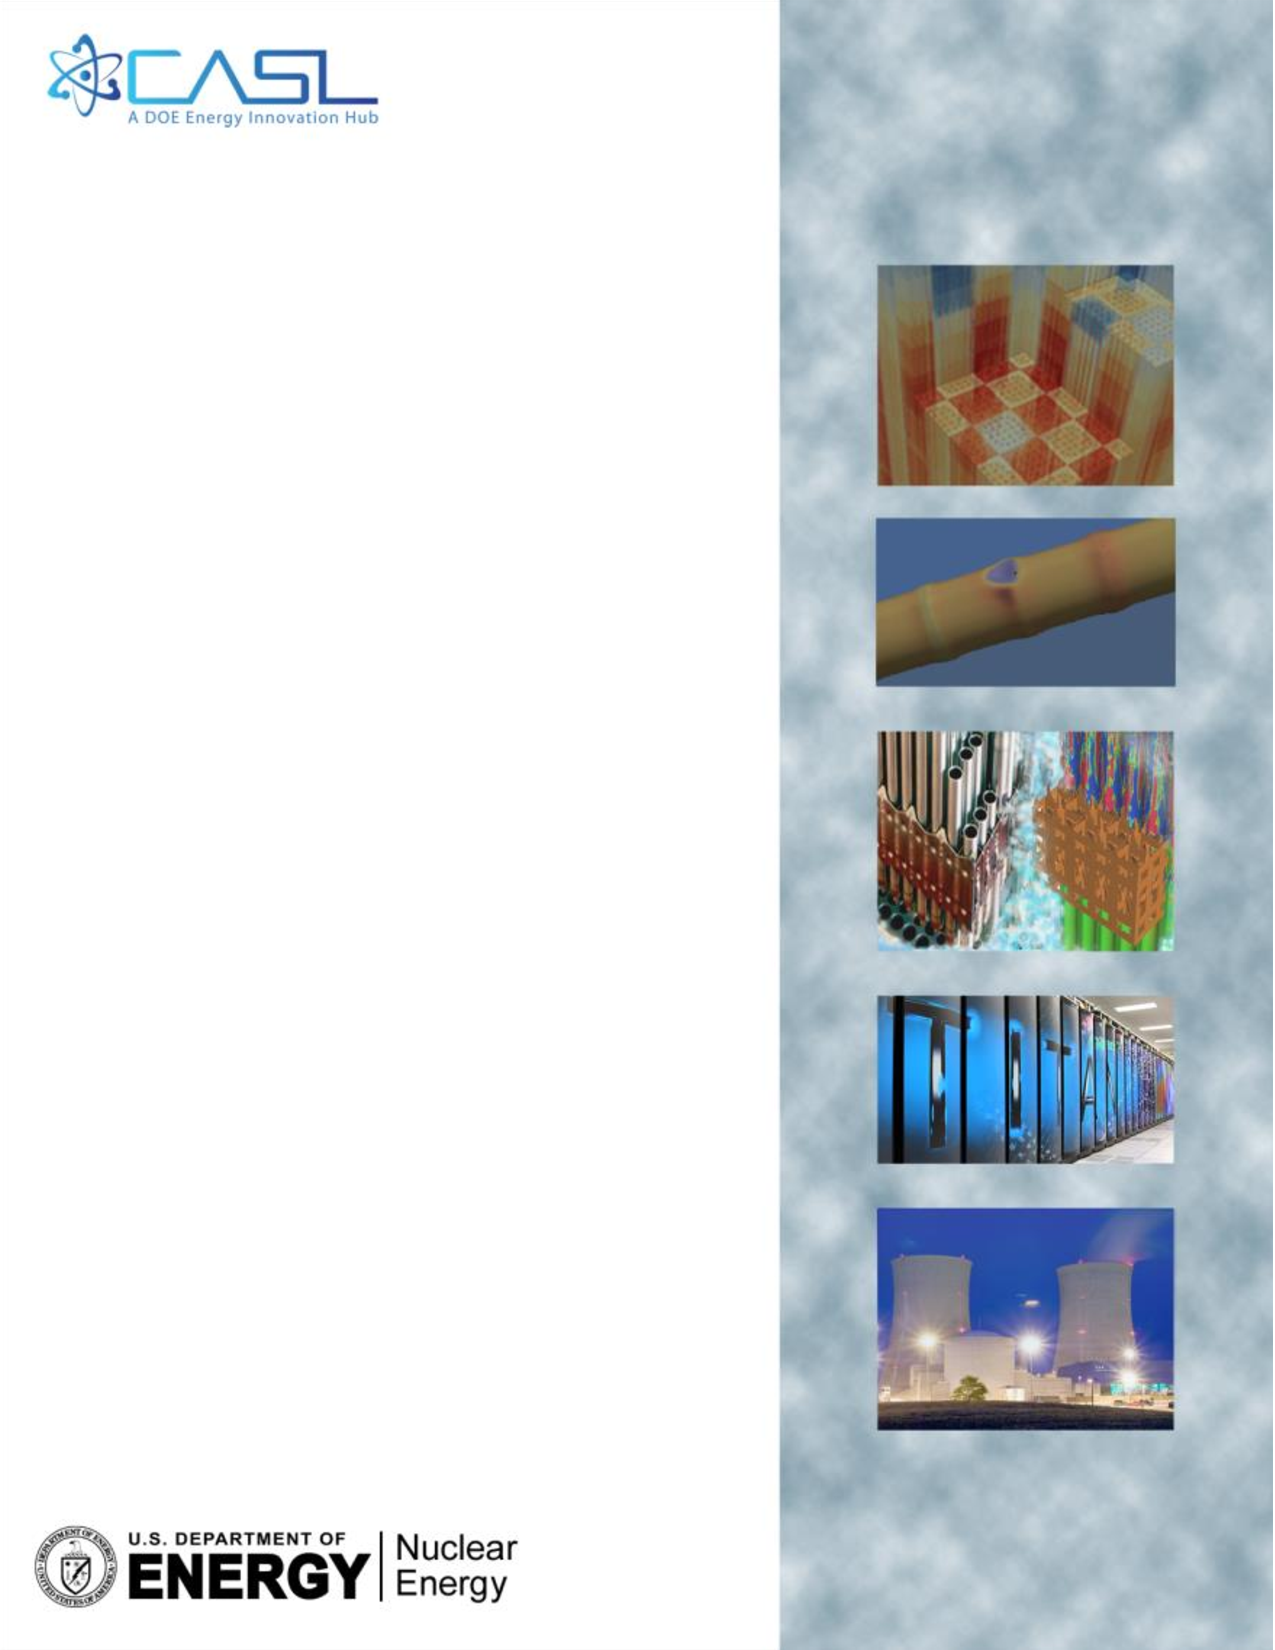
\includegraphics[width=\paperwidth,height=\paperheight]{template/casl_background.pdf}
  }%
}

% Define command to surround text in angle brackets
\newcommand{\brackets}[1]{\textlangle{}#1\textrangle{}}

% For formatting code
\newcommand{\codeblock}[1]{\texttt{#1}}

%increase space after captions
\setlength{\belowcaptionskip}{2pt}

% No indenting at start of paragraph
\setlength{\parindent}{0pt}

%increase space between paragraphs
\parskip 1em

\titleformat{\chapter}{\Huge\bfseries}{\thechapter. }{0pt}{\Huge\bfseries}

% set the section numbering depth and TOC depth
\setcounter{secnumdepth}{3}
\setcounter{tocdepth}{3}

% Use continuous counting scheme for floats
\counterwithout{table}{chapter}

\let\DeclareUSUnit\DeclareSIUnit
\let\US\SI
\DeclareUSUnit\F{F}
\DeclareUSUnit\ft{ft}
\DeclareSIUnit\inch{in}

%define the degree command for using temperature units
\providecommand{\degree}{\ensuremath{^{\circ}}}

% define new command to make custom vector notation
\newcommand{\vect}[1]{\vec{#1}}

% define a command to correct subscript size
\newcommand{\smallsub}[1]{\scriptscriptstyle{\text{#1}}}

% Define a macro to make the "by" symbol 
\newcommand{\by}{\texorpdfstring{\ensuremath{\times}}{x}}

% define command for quick scientific notation
\providecommand{\e}[1]{\ensuremath{\cdot10^{#1}}}

\usepackage{todonotes}

\newcommand*{\Appendixautorefname}{Appendix}


\title{VERAIn Software Requirements, Test Plan, and Test Report}
\newcommand{\shortTitle}{Test plan, report, and requirements}
\newcommand{\subtitle}{}
\newcommand{\CASLMilestoneNumber}{CASL-U-2019-1891-000}
\newcommand{\publicationDate}{7/31/2019}
\newcommand{\psm}{Scott Palmtag, VERAIn Product Software Manager}
\newcommand{\reviewer}{Independent Reviewer}

\author[1]{Erik Walker}

\affil[1]{Oak Ridge National Laboratory}


\addbibresource{biblio.bib}


\begin{document}

% CASL front matter uses roman numerals
\pagenumbering{roman}

\begin{titlepage}

   \BgThispage
   \thispagestyle{firststyle}
   
   \vspace*{\fill}
   
   \begin{minipage}[l][][c]{0.6\textwidth}
   \begin{flushleft}
   \makeatletter
   {\huge\color{TitleBlue}\bf Consortium for Advanced \\\vspace{0.3cm} Simulation of LWRs}\\
   \vspace{3cm}
   {\huge\fontfamily{phv}\selectfont\color{TitleBlue}\bf
   % Title of the document
   \@title\par
   }
   {\Large\fontfamily{phv}\selectfont\color{DocNameBlue}\bf
   \subtitle\par
   }
   \vspace*{30pt}
   % Authors
   {\Large\bf\setlength{\parskip}{10pt}
   \@author
   
   }
   \vspace*{30pt}
   {\huge\bf
   \publicationDate
   }
   \makeatother
   
   
   \end{flushleft}
   \end{minipage}
   
   \vspace*{\fill}
   
\begin{minipage}{0.6\textwidth}
   
\includegraphics[width=\textwidth]{template/verabanner.png}
\end{minipage}

   
   \end{titlepage}

   \pagestyle{fancy}

   \vspace*{\fill}

   \captionsetup{justification=centering}
   \begin{table}[H]
   \centering
   \caption*{\Large\bfseries{Revision Log}}
   \begin{tabular}{rrrr}
   \toprule
   \textbf{Revision} & \textbf{Date} & \textbf{Affected Pages} & \textbf{Revision Description} \\
   \midrule
   0 & 7/31/2019 & All & Initial Release \\
   1 & 11/15/2019 & All & 4.1 Release \\
   & & & \\
   & & & \\
   & & & \\
   & & & \\
   & & & \\
   \bottomrule
   \end{tabular}
   \end{table}
   
   \vspace*{\fill}
   
   
   \begin{table}[H]
   \caption*{\Large\bfseries{Document pages that are:}}
   \centering
   \begin{tabular}{ll}
   Export Controlled: & None \\
   IP/Proprietary/NDA Controlled: & None \\
   Sensitive Controlled: & None \\
   Unlimited: & All \\
   \end{tabular}
   \end{table}
   
   \vspace*{\fill}
   
   This document was prepared as an account of work sponsored by an agency of the United States Government. Neither the United States Government nor any agency thereof, nor any of their employees, makes any warranty, express or implied, or assumes any legal liability or responsibility for the accuracy, completeness, or usefulness of any information, apparatus, product, or process disclosed, or represents that its use would not infringe privately owned rights. Reference herein to any specific commercial product, process, or service by trade name, trademark, manufacturer, or otherwise, does not necessarily constitute or imply its endorsement, recommendation, or favoring by the United States Government or any agency thereof. The views and opinions of authors expressed herein do not necessarily state or reflect those of the United States Government or any agency thereof.

   \captionsetup{justification=justified}
   
   \vspace*{\fill}

\pagestyle{fancy}
\clearpage 

\makeatletter
\begin{center}
{\huge\bf\@title\par}
\end{center}

\vspace{2cm}

{\Large\bf Approvals:}

\vspace{2cm}

\begin{tabular}{ll}
\makebox[3.5in]{\hrulefill} & \makebox[2.0in]{\hrulefill}\\
{\bf\psm} & {\bf Date}\\[3cm]
\makebox[3.5in]{\hrulefill} & \makebox[2.0in]{\hrulefill}\\
{\bf\reviewer} & {\bf Date}\\[3cm]
\end{tabular}

\makeatother

\clearpage


% The CASL title page is 2 pages long and will be attached to the front
% of this document
%\setcounter{page}{3}

% CASL front-matter headers are centered
%\sectionfont{\centering}

%\listoftodos

\addcontentsline{toc}{section}{Executive Summary}
\chapter*{Executive Summary}

This document describes the software test plan for VERAIn and provides appendices for the software requirements and software test report.
In this document, the test platform hardware and software are described.
Section \ref{sec:A1} provides a list of the tests run and their acceptability as a test report.
Section \ref{sec:A2} provides the list of low-level software requirements as a requirements traceability matrix.

%\newpage
%\begin{center}
%(This page intentionally left blank)
%\end{center}
%{\pagestyle{empty}\cleardoublepage }

%\renewcommand{\contentsname}{CONTENTS}
%\addcontentsline{toc}{chapter}{CONTENTS}
\tableofcontents

%\begin{center}
%(This page intentionally left blank)
%\end{center}
%{\pagestyle{empty}\cleardoublepage }

%\renewcommand{\listfigurename}{FIGURES}
%\addcontentsline{toc}{section}{FIGURES} 
%\listoffigures

%\renewcommand{\listtablename}{TABLES}
%\addcontentsline{toc}{section}{TABLES} 
\listoftables

%\newpage

%\addcontentsline{toc}{section}{Acronyms} 
%\chapter*{Acronyms}

\begin{acronym}
  \acro{1D}[1D]{one-dimensional}
  \acro{2D}[2D]{two-dimensional}
  \acro{3D}[3D]{three-dimensional}
  \acro{ama}[AMA]{Advanced Modeling Applications}
  \acro{api}[API]{application interface}
  \acro{bfbt}[BFBT]{BWR fine-mesh bundle tests}
  \acro{bwr}[BWR]{boiling water reactor}
  \acro{cad}[CAD]{computer-aided drafting}
  \acro{casl}[CASL]{Consortium for Advanced Simulation of Light Water
  Reactors}
  \acro{ce}[CE]{Combustion Engineering}
  \acro{cea}[CEA]{Commissariat \`a l'\'energie atomique}
  \acro{cilc}[CILC]{crud-induced localized corrosion}
  \acro{fy}[FY]{fiscal year}
  \acro{cfd}[CFD]{computational fluid dynamics}
  \acro{chf}[CHF]{critical heat flux}
  \acro{cips}[CIPS]{crud-induced power shift}
  \acro{dnb}[DNB]{departure from nucleate boiling}
  \acro{edf}[EDF]{\'Electricit\'e de France}
  \acro{efpd}[EFPD]{effective full power days}
  \acro{eohl}[EOHL]{end of heated length}
  \acro{epri}[EPRI]{Electric Power Research Institute}
  \acro{farea}[FA]{focus area}
  \acro{fmc}[FMC]{Fuels, Materials, and Chemistry \ac{farea}}
  \acro{gsce}[GSCE]{grid-spacer cooling enhancement}
  \acro{hdf5}[HDF5]{Hierarchical Data Format 5}
  \acro{hn}[HN]{Hancox--Nicoll}
  \acro{htc}[HTC]{heat transfer coefficient}
  \acro{ifba}[IFBA]{integral fuel burnable absorber}
  \acro{ldv}[LDV]{laser doppler velocimetry}
  \acro{lwr}[LWR]{light water reactor}
  \acro{mit}[MIT]{Massachusetts Institute of Technology}
  \acro{mvg}[MVG]{mixing vane grid}
  \acro{nda}[NDA]{nondisclosure agreement}
  \acro{nestor}[NESTOR]{New Experimental Studies on Rod Bundles}
  \acro{nist}[NIST]{National Institute of Standards and Technology}
  \acro{nrc}[NRC]{US Nuclear Regulatory Commission}
  \acro{onb}[ONB]{onset of nucleate boiling}
  \acro{ornl}[ORNL]{Oak Ridge National Laboratory}
  \acro{psbt}[PSBT]{PWR subchannel and bundle tests}
  \acro{pwr}[PWR]{pressurized water reactor}
  \acro{phi}[PHI]{physics-integration focus area}
  \acro{rms}[RMS]{root-mean-square}
  \acro{rmse}[RMSE]{root-mean-square error}
  \acro{rothcon}[ROTHCON]{rod thermal hydraulic reconstruction}
  \acro{rRMSE}[rRMSE]{relative root-mean-square error}
  \acro{ssg}[SSG]{simple support grid}
  \acro{th}[T/H]{thermal-hydraulics}
  \acro{thm}[THM]{thermal-hydraulics methods focus area}
  \acro{tke}[TKE]{turbulent kinetic energy}
  \acro{TRACE}[TRACE]{TRAC/RELAP Advanced Computational Engine}
  \acro{verain}[VERAIn]{VERA-CS common input file}
  \acro{vv}[V\&V]{verification and validation}
  \acro{wec}[WEC]{Westinghouse Electric Company}
  \acro{yhl}[YHL]{Yao--Hochreiter--Leech}
\end{acronym}

%\textbf{Acknowledgements:}  This work is supported by the
%Consortium for Advanced Simulation of Light Water Reactors
%(www.casl.gov), an Energy Innovation Hub for Modeling and Simulation of
%Nuclear Reactors under US Department of Energy Contract No.
%DE-AC05-00OR22725.
	
\newpage

\acresetall

\newpage

%\begin{center}
%(This page intentionally left blank)
%\end{center}
%{\pagestyle{empty}\cleardoublepage }

\pagenumbering{arabic}

% Return section headers to left-justified
\sectionfont{}

%\todo{remove fig, table, etc. pages}
%\todo{possibly combine nomenclature page with nomenclature table}

\chapter{Testing Procedure}
\label{sec:test_procedure}

\section{Computer Program Tested}
\subsection{Program: VERAIn}
Built under VERA Environment with following packages and versions:
\lstinputlisting[caption={Software Versions Evaluated},label={lst:repos}]{VERARepoVersions.txt}

VERAIn has no dependencies on any other code package contained within VERA.

\subsection{System Software}
The operating system on which these tests were performed was: Linux 3.10.0-957.21.3.el7.x86\_64 .
\subsection{Test Calibration}
None.
\subsection{Computer Hardware used for Testing}
james007.ornl.gov
\section{Test Equipment Calibration}
None.
\section{Date of Test}
Started: Aug 10, 2019 - 01:19 UTC\\
Total Test Time: 2 minutes, 40 seconds
\section{Data Recorder}
CTest-3.10.2 and CDash Version trilinos-release-2018-08-prebuilt
\section{Simulation Models Used}
Since VERAIn is only an input parser, it contains no simulation models.
\section{Test Problems}
A list of test problems and their requirements may be found in Section \ref{sec:A2} of this document.
\section{Results and Applicability}
\subsection*{Results}
Results are given in Section \ref{sec:A1}.
\subsection*{Applicability}
The test results from Section \ref{sec:A1} satisfy the requirements defined in the software requirements. 
\section{Action Taken in Connection with Noted Deviations}
There were no noted deviations. Therefore, no actions were taken.
\subsection{Person Evaluating Results}
Erik Walker
\section{Acceptability}
The acceptance criterion is that all tests pass their individual criteria. As evidenced in column 4 of the table in Section \ref{sec:A1}, all tests passed their criteria.
The primary type of test performed in the VERAIn test matrix are regression tests that compare a test output file to a version-controlled reference file deemed to be correct.

Regression test reference files are XML.gold files that have been generated and reviewed for correctness.
Once the VERAIn parser is run on an input, the resulting XML file is compared to the corresponding XML.gold file using a straight diff. If the files are identical, then the test passes. If any differences exist in the files, the test fails. 

There are also a few tests that are designed to intentionally fail. These tests are intended to capture common input mistakes and ensure that the parser fails hard when these mistakes are encountered. 

The test results were reviewed by the Product Support Manager and the Independent Technical Reviewer who have determined that the computer program is acceptable for integration with the VERA Product Suite.
The test results have demonstrated the computer program(s) adequately and correctly performed.
The testing covered the specified software requirements, proper handling of abnormal conditions or events, and interfaces with other components. 
The testing verified the computer program did not introduce unintended consequences which degraded the overall software function. 
No discrepancies between expected and observed software functioning were identified.

\chapter{Applicable Standards and Procedures}
\begin{itemize}
    \item NQA-1-2008 with NQA-1a-2009 Addenda \cite{NQA12008}
    \item VERA-QA-004, VERA Software Configuration and Control
    \item VERA-QA-006, VERA Software Requirements, Design, and Testing
\end{itemize}
\chapter{Required Records}
\section{CDash Test Results}
See Section \ref{sec:A1}.
\section{Requirements Traceability Matrix}
See Section \ref{sec:A2}.

\clearpage
%\titleformat{\section}{\bf\large}{\appendixname~\thetitle}{1ex}[]
\begin{appendices}
    \chapter{VERAIn Test Report}
    \label{sec:A1}
    The following table was obtained from a CDash report.
    CDash is a web application included with CMake and CTest.
    CMake is the VERA build system and CTest is a program for automatically running tests defined with CMake and sending results to CDash.
    All tests are included in the Git repositories noted in List \ref{lst:repos}.
    Section \ref{sec:A2} provides a list of the test names along with the test input files and requirements.
    \begin{longtable}[!ht]{|p{0.75cm}|p{11.25cm}|p{1.6cm}|p{1.1cm}|}
\caption{VERAIn Test Report from \href{https://casl-dev.ornl.gov/cdash/viewTest.php?buildid=149707}{CDash} }\label{tab:str} \\

\hline
\rowcolor{CASLBlue}
\color{white}\textbf{No.} & \color{white}\textbf{Test Name} & \color{white}\textbf{Details} & \color{white}\textbf{Status} \\
\hline
\endfirsthead
\hline
\rowcolor{CASLBlue}
\color{white}\textbf{No.} & \color{white}\textbf{Test Name} & \color{white}\textbf{Details} & \color{white}\textbf{Status} \\
\hline
\endhead
\hline
\endfoot
\hline
\endlastfoot


\rowcolor{caslcolor1}\small 1 & \small VERAIn\_react2xml\_bwr-peach-2 & \small Completed & \small Passed \\\hline
\rowcolor{caslcolor2}\small 2 & \small VERAIn\_react2xml\_bwr-peach-1 & \small Completed & \small Passed \\\hline
\rowcolor{caslcolor1}\small 3 & \small VERAIn\_react2xml\_bwr-peach-4 & \small Completed & \small Passed \\\hline
\rowcolor{caslcolor2}\small 4 & \small VERAIn\_react2xml\_bwr-ge9 & \small Completed & \small Passed \\\hline
\rowcolor{caslcolor1}\small 5 & \small VERAIn\_react2xml\_bwr-peach-5 & \small Completed & \small Passed \\\hline
\rowcolor{caslcolor2}\small 6 & \small VERAIn\_react2xml\_bwr-peach-3 & \small Completed & \small Passed \\\hline
\rowcolor{caslcolor1}\small 7 & \small VERAIn\_react2xml\_bwr-thickthincb & \small Completed & \small Passed \\\hline
\rowcolor{caslcolor2}\small 8 & \small VERAIn\_react2xml\_bwr-peach-6 & \small Completed & \small Passed \\\hline
\rowcolor{caslcolor1}\small 9 & \small VERAIn\_react2xml\_bwr-plr & \small Completed & \small Passed \\\hline
\rowcolor{caslcolor2}\small 10 & \small VERAIn\_react2xml\_bwr-azixs & \small Completed & \small Passed \\\hline
\rowcolor{caslcolor1}\small 11 & \small VERAIn\_react2xml\_bwr-hetblade & \small Completed & \small Passed \\\hline
\rowcolor{caslcolor2}\small 12 & \small VERAIn\_react2xml\_bwr-p6-test & \small Completed & \small Passed \\\hline
\rowcolor{caslcolor1}\small 13 & \small VERAIn\_react2xml\_bwr\_jagged & \small Completed & \small Passed \\\hline
\rowcolor{caslcolor2}\small 14 & \small VERAIn\_react2xml\_bwr-axialvoid & \small Completed & \small Passed \\\hline
\rowcolor{caslcolor1}\small 15 & \small VERAIn\_react2xml\_ex7\_bwr & \small Completed & \small Passed \\\hline
\rowcolor{caslcolor2}\small 16 & \small VERAIn\_react2xml\_apr1400-cyc1 & \small Completed & \small Passed \\\hline
\rowcolor{caslcolor1}\small 17 & \small VERAIn\_react2xml\_FAST\_input\_block & \small Completed & \small Passed \\\hline
\rowcolor{caslcolor2}\small 18 & \small VERAIn\_react2xml\_chen\_3x3 & \small Completed & \small Passed \\\hline
\rowcolor{caslcolor1}\small 19 & \small VERAIn\_react2xml\_cross\_w\_baffle & \small Completed & \small Passed \\\hline
\rowcolor{caslcolor2}\small 20 & \small VERAIn\_react2xml\_MSED & \small Completed & \small Passed \\\hline
\rowcolor{caslcolor1}\small 21 & \small VERAIn\_react2xml\_default\_density\_change & \small Completed & \small Passed \\\hline
\rowcolor{caslcolor2}\small 22 & \small VERAIn\_react2xml\_fast\_3x3rod\_HFP & \small Completed & \small Passed \\\hline
\rowcolor{caslcolor1}\small 23 & \small VERAIn\_react2xml\_p6a\_sa\_1300\_vuq & \small Completed & \small Passed \\\hline
\rowcolor{caslcolor2}\small 24 & \small VERAIn\_react2xml\_mspc & \small Completed & \small Passed \\\hline
\rowcolor{caslcolor1}\small 25 & \small VERAIn\_react2xml\_fuel\_options & \small Completed & \small Passed \\\hline
\rowcolor{caslcolor2}\small 26 & \small VERAIn\_react2xml\_ctf\_convergence\_terms & \small Completed & \small Passed \\\hline
\rowcolor{caslcolor1}\small 27 & \small VERAIn\_react2xml\_mox1 & \small Completed & \small Passed \\\hline
\rowcolor{caslcolor2}\small 28 & \small VERAIn\_react2xml\_mamba\_mass\_bal & \small Completed & \small Passed \\\hline
\rowcolor{caslcolor1}\small 29 & \small VERAIn\_react2xml\_detector\_edits & \small Completed & \small Passed \\\hline
\rowcolor{caslcolor2}\small 30 & \small VERAIn\_react2xml\_par\_cross & \small Completed & \small Passed \\\hline
\rowcolor{caslcolor1}\small 31 & \small VERAIn\_react2xml\_misc\_options & \small Completed & \small Passed \\\hline
\rowcolor{caslcolor2}\small 32 & \small VERAIn\_react2xml\_pwr-CE-2a & \small Completed & \small Passed \\\hline
\rowcolor{caslcolor1}\small 33 & \small VERAIn\_react2xml\_pwr\_CE\_single\_16x16 & \small Completed & \small Passed \\\hline
\rowcolor{caslcolor2}\small 34 & \small VERAIn\_react2xml\_pwr-CE-2b & \small Completed & \small Passed \\\hline
\rowcolor{caslcolor1}\small 35 & \small VERAIn\_react2xml\_Sample\_3x3 & \small Completed & \small Passed \\\hline
\rowcolor{caslcolor2}\small 36 & \small VERAIn\_react2xml\_Sample\_7x7 & \small Completed & \small Passed \\\hline
\rowcolor{caslcolor1}\small 37 & \small VERAIn\_react2xml\_Sample\_3x3\_multistate & \small Completed & \small Passed \\\hline
\rowcolor{caslcolor2}\small 38 & \small VERAIn\_react2xml\_Sample\_full\_core\_maps & \small Completed & \small Passed \\\hline
\rowcolor{caslcolor1}\small 39 & \small VERAIn\_react2xml\_Sample\_full\_core & \small Completed & \small Passed \\\hline
\rowcolor{caslcolor2}\small 40 & \small VERAIn\_react2xml\_Sample\_full\_core\_matmix & \small Completed & \small Passed \\\hline
\rowcolor{caslcolor1}\small 41 & \small VERAIn\_react2xml\_Sample\_full\_core\_wsym\_assm\_even & \small Completed & \small Passed \\\hline
\rowcolor{caslcolor2}\small 42 & \small VERAIn\_react2xml\_Sample\_full\_core\_fuelmix & \small Completed & \small Passed \\\hline
\rowcolor{caslcolor1}\small 43 & \small VERAIn\_react2xml\_Sample\_full\_core\_reflector & \small Completed & \small Passed \\\hline
\rowcolor{caslcolor2}\small 44 & \small VERAIn\_react2xml\_Sample\_full\_core\_wsym & \small Completed & \small Passed \\\hline
\rowcolor{caslcolor1}\small 45 & \small VERAIn\_react2xml\_Sample\_full\_core\_wsym\_even & \small Completed & \small Passed \\\hline
\rowcolor{caslcolor2}\small 46 & \small VERAIn\_react2xml\_Sample\_full\_core\_wsym\_state\_assm & \small Completed & \small Passed \\\hline
\rowcolor{caslcolor1}\small 47 & \small VERAIn\_react2xml\_Sample\_full\_core\_wsym\_state\_dsym & \small Completed & \small Passed \\\hline
\rowcolor{caslcolor2}\small 48 & \small VERAIn\_react2xml\_Sample\_full\_core\_wsym\_state\_assm\_matopt & \small Completed & \small Passed \\\hline
\rowcolor{caslcolor1}\small 49 & \small VERAIn\_react2xml\_Sample\_p3 & \small Completed & \small Passed \\\hline
\rowcolor{caslcolor2}\small 50 & \small VERAIn\_react2xml\_Sample\_p3\_Anderson & \small Completed & \small Passed \\\hline
\rowcolor{caslcolor1}\small 51 & \small VERAIn\_react2xml\_Sample\_p3\_mpact & \small Completed & \small Passed \\\hline
\rowcolor{caslcolor2}\small 52 & \small VERAIn\_react2xml\_Sample\_p3\_unit\_test & \small Completed & \small Passed \\\hline
\rowcolor{caslcolor1}\small 53 & \small VERAIn\_react2xml\_Sample\_p4a\_unit\_test & \small Completed & \small Passed \\\hline
\rowcolor{caslcolor2}\small 54 & \small VERAIn\_react2xml\_Sample\_full\_core\_wsym\_state & \small Completed & \small Passed \\\hline
\rowcolor{caslcolor1}\small 55 & \small VERAIn\_react2xml\_Sample\_p4 & \small Completed & \small Passed \\\hline
\rowcolor{caslcolor2}\small 56 & \small VERAIn\_react2xml\_Sample\_p6a & \small Completed & \small Passed \\\hline
\rowcolor{caslcolor1}\small 57 & \small VERAIn\_react2xml\_Sample\_p6a\_multifuel & \small Completed & \small Passed \\\hline
\rowcolor{caslcolor2}\small 58 & \small VERAIn\_react2xml\_Sample\_p4\_mpact & \small Completed & \small Passed \\\hline
\rowcolor{caslcolor1}\small 59 & \small VERAIn\_react2xml\_Sample\_p7 & \small Completed & \small Passed \\\hline
\rowcolor{caslcolor2}\small 60 & \small VERAIn\_react2xml\_Seabrook\_5x5rod\_HFP & \small Completed & \small Passed \\\hline
\rowcolor{caslcolor1}\small 61 & \small VERAIn\_react2xml\_Sample\_qtr\_core\_wsym\_3x3\_standalone & \small Completed & \small Passed \\\hline
\rowcolor{caslcolor2}\small 62 & \small VERAIn\_react2xml\_Sample\_p9\_shuffle & \small Completed & \small Passed \\\hline
\rowcolor{caslcolor1}\small 63 & \small VERAIn\_react2xml\_Sample\_p9\_restart & \small Completed & \small Passed \\\hline
\rowcolor{caslcolor2}\small 64 & \small VERAIn\_react2xml\_Sample\_p9\_jumpin & \small Completed & \small Passed \\\hline
\rowcolor{caslcolor1}\small 65 & \small VERAIn\_react2xml\_small\_3x3rod\_Bison & \small Completed & \small Passed \\\hline
\rowcolor{caslcolor2}\small 66 & \small VERAIn\_react2xml\_small\_3x3rod\_HFP\_2fuel & \small Completed & \small Passed \\\hline
\rowcolor{caslcolor1}\small 67 & \small VERAIn\_react2xml\_small\_3x3rod\_Bison\_standalone & \small Completed & \small Passed \\\hline
\rowcolor{caslcolor2}\small 68 & \small VERAIn\_react2xml\_small\_3x3rod\_BProd & \small Completed & \small Passed \\\hline
\rowcolor{caslcolor1}\small 69 & \small VERAIn\_react2xml\_small\_3x3rod\_HFP & \small Completed & \small Passed \\\hline
\rowcolor{caslcolor2}\small 70 & \small VERAIn\_react2xml\_small\_3x3rod\_HFP\_8g & \small Completed & \small Passed \\\hline
\rowcolor{caslcolor1}\small 71 & \small VERAIn\_react2xml\_small\_3x3rod\_HZP & \small Completed & \small Passed \\\hline
\rowcolor{caslcolor2}\small 72 & \small VERAIn\_react2xml\_small\_5cross\_assem\_3x3rod\_HFP & \small Completed & \small Passed \\\hline
\rowcolor{caslcolor1}\small 73 & \small VERAIn\_react2xml\_small\_multibundle & \small Completed & \small Passed \\\hline
\rowcolor{caslcolor2}\small 74 & \small VERAIn\_react2xml\_small\_3x3rod\_IFBA & \small Completed & \small Passed \\\hline
\rowcolor{caslcolor1}\small 75 & \small VERAIn\_react2xml\_small\_qtr\_core\_3x3rod\_HFP & \small Completed & \small Passed \\\hline
\rowcolor{caslcolor2}\small 76 & \small VERAIn\_react2xml\_small\_multibundle\_par & \small Completed & \small Passed \\\hline
\rowcolor{caslcolor1}\small 77 & \small VERAIn\_react2xml\_small\_singlerod\_HFP\_8gb & \small Completed & \small Passed \\\hline
\rowcolor{caslcolor2}\small 78 & \small VERAIn\_react2xml\_small\_singlerod\_HFP\_8g & \small Completed & \small Passed \\\hline
\rowcolor{caslcolor1}\small 79 & \small VERAIn\_react2xml\_small\_singlerod\_HFP & \small Completed & \small Passed \\\hline
\rowcolor{caslcolor2}\small 80 & \small VERAIn\_react2xml\_5cross\_nodal\_par\_qtr & \small Completed & \small Passed \\\hline
\rowcolor{caslcolor1}\small 81 & \small VERAIn\_react2xml\_decreasing-axial & \small Completed & \small Passed \\\hline
\rowcolor{caslcolor2}\small 82 & \small VERAIn\_react2xml\_front-dash & \small Completed & \small Passed \\\hline
\rowcolor{caslcolor1}\small 83 & \small VERAIn\_react2xml\_disable\_xml2ctf & \small Completed & \small Passed \\\hline
\rowcolor{caslcolor2}\small 84 & \small VERAIn\_veradiff\_match & \small Completed & \small Passed \\\hline
\rowcolor{caslcolor1}\small 85 & \small VERAIn\_veradiff\_fail & \small Completed & \small Passed \\\hline
\rowcolor{caslcolor2}\small 86 & \small VERAIn\_react2xml\_test\_cobra\_edits & \small Completed & \small Passed \\\hline
\rowcolor{caslcolor1}\small 87 & \small VERAIn\_react2xml\_test\_cobra\_edits\_inimat & \small Completed & \small Passed \\\hline
\rowcolor{caslcolor2}\small 88 & \small VERAIn\_react2xml\_test\_verashift\_3a & \small Completed & \small Passed \\\hline
\rowcolor{caslcolor1}\small 89 & \small VERAIn\_react2xml\_test-short & \small Completed & \small Passed \\\hline
\rowcolor{caslcolor2}\small 90 & \small VERAIn\_react2xml\_test\_verashift\_3a\_forward & \small Completed & \small Passed \\\hline
\rowcolor{caslcolor1}\small 91 & \small VERAIn\_react2xml\_smr-7x7 & \small Completed & \small Passed \\\hline
\rowcolor{caslcolor2}\small 92 & \small VERAIn\_react2xml\_test\_verashift\_3a\_cadis & \small Completed & \small Passed \\\hline
\rowcolor{caslcolor1}\small 93 & \small VERAIn\_react2xml\_with-dash & \small Completed & \small Passed \\\hline
\rowcolor{caslcolor2}\small 94 & \small VERAIn\_react2xml\_test\_verashift\_4mini\_nonunique & \small Completed & \small Passed \\\hline
\rowcolor{caslcolor1}\small 95 & \small VERAIn\_react2xml\_2a\_LS & \small Completed & \small Passed \\\hline
\rowcolor{caslcolor2}\small 96 & \small VERAIn\_react2xml\_2a\_LS\_default & \small Completed & \small Passed \\\hline
\rowcolor{caslcolor1}\small 97 & \small VERAIn\_react2xml\_5cross\_multiassem & \small Completed & \small Passed \\\hline
\rowcolor{caslcolor2}\small 98 & \small VERAIn\_react2xml\_multi\_scalar\_error & \small Completed & \small Passed \\\hline
\rowcolor{caslcolor1}\small 99 & \small VERAIn\_react2xml\_test\_verashift\_small\_core\_bioshield\_no\_pv & \small Completed & \small Passed \\\hline
\rowcolor{caslcolor2}\small 100 & \small VERAIn\_react2xml\_test\_verashift\_4mini\_nonunique\_bioshield & \small Completed & \small Passed \\\hline
\rowcolor{caslcolor1}\small 101 & \small VERAIn\_xmlthexp\_Sample\_p6a & \small Completed & \small Passed \\\hline
\rowcolor{caslcolor2}\small 102 & \small VERAIn\_react2xml\_test\_verashift\_small\_core\_bioshield & \small Completed & \small Passed \\\hline
\rowcolor{caslcolor1}\small 103 & \small VERAIn\_testVERAInMan & \small Completed & \small Passed \\\hline



\end{longtable}

    \clearpage
    
    \chapter{Requirements and Test Traceability Matrix}
    \label{sec:A2}
    For the entries in the Additional Info field, the \#NNNN is the CASL PHI Kanban ticket number with a hyperlink to this webpage.
    \begin{longtable}[!ht]{|p{1.4cm}|p{14cm}|}
\caption{Requirements}\label{tab:req}\\

\hline
\multirow{4}{*}{\textbf{Req. ID}} & \cellcolor{caslheader}\textcolor{white}{\textit{Requirement Description}} \\\cline{2-2}
                   & \cellcolor{caslcolor1} \textit{Test Name} \\\cline{2-2}
                   & \cellcolor{caslcolor2} \textit{Test Input} \\\cline{2-2}
                   & \cellcolor{caslcolor1} \textit{Additional Info} \\\hline
\endfirsthead

\hline
\multirow{4}{*}{\textbf{Req. ID}} & \cellcolor{caslheader}\textcolor{white}{\textit{Requirement Description}} \\\cline{2-2}
                   & \cellcolor{caslcolor1} \textit{Test Name} \\\cline{2-2}
                   & \cellcolor{caslcolor2} \textit{Test Input} \\\cline{2-2}
                   & \cellcolor{caslcolor1} \textit{Additional Info} \\\hline
\endhead
\hline
\endfoot
\hline
\endlastfoot

\multirow{4}{*}{1} & \cellcolor{caslheader}\textcolor{white}{The VERAIn package shall be able to parse VERA Progression Problem 2A with specified linear source options} \\\cline{2-2}

                   & \cellcolor{caslcolor2}verain/test/2a\_LS.inp \\\cline{2-2}
                   & \cellcolor{caslcolor1}None \\\hline
\multirow{4}{*}{2} & \cellcolor{caslheader}\textcolor{white}{The VERAIn package shall be able to parse VERA Progression Problem 2A with default linear source options} \\\cline{2-2}

                   & \cellcolor{caslcolor2}verain/test/2a\_LS\_default.inp \\\cline{2-2}
                   & \cellcolor{caslcolor1}None \\\hline
\multirow{4}{*}{3} & \cellcolor{caslheader}\textcolor{white}{The VERAIn package shall be able to parse all FAST input options correctly} \\\cline{2-2}

                   & \cellcolor{caslcolor2}verain/test/FAST\_input\_block.inp \\\cline{2-2}
                   & \cellcolor{caslcolor1}None \\\hline
\multirow{4}{*}{4} & \cellcolor{caslheader}\textcolor{white}{The VERAIn package shall be able to parse inputs in which multigrid solver
 options are specified} \\\cline{2-2}

                   & \cellcolor{caslcolor2}verain/test/MSED.inp \\\cline{2-2}
                   & \cellcolor{caslcolor1}None \\\hline
\multirow{4}{*}{5} & \cellcolor{caslheader}\textcolor{white}{The VERAIn package shall be able to parse a full 3D core with an even 
   core size} \\\cline{2-2}

                   & \cellcolor{caslcolor2}verain/test/S\_even.inp \\\cline{2-2}
                   & \cellcolor{caslcolor1}None \\\hline
\newpage\multirow{4}{*}{6} & \cellcolor{caslheader}\textcolor{white}{The VERAIn package shall be able to parse 9 3D 17x17 assemblies with feedback
 enabled in full symmetry} \\\cline{2-2}

                   & \cellcolor{caslcolor2}verain/test/Sample\_3x3.inp \\\cline{2-2}
                   & \cellcolor{caslcolor1}None \\\hline
\multirow{4}{*}{7} & \cellcolor{caslheader}\textcolor{white}{The VERAIn package shall be able to parse multiple state blocks containing
 differing options selected for the tinlet card and table input for inlet temperature as a function of power} \\\cline{2-2}

                   & \cellcolor{caslcolor2}verain/test/Sample\_3x3\_multistate.inp \\\cline{2-2}
                   & \cellcolor{caslcolor1}None \\\hline
\multirow{4}{*}{8} & \cellcolor{caslheader}\textcolor{white}{The VERAIn package shall be able to parse 49 3D 17x17 assemblies with feedback
 enabled in full symmetry} \\\cline{2-2}

                   & \cellcolor{caslcolor2}verain/test/Sample\_7x7.inp \\\cline{2-2}
                   & \cellcolor{caslcolor1}None \\\hline
\multirow{4}{*}{9} & \cellcolor{caslheader}\textcolor{white}{The VERAIn package shall be able to parse a full 3D core} \\\cline{2-2}

                   & \cellcolor{caslcolor2}verain/test/Sample\_full\_core.inp \\\cline{2-2}
                   & \cellcolor{caslcolor1}None \\\hline
\multirow{4}{*}{10} & \cellcolor{caslheader}\textcolor{white}{The VERAIn package shall be able to parse a full 3D core with fuel mixing} \\\cline{2-2}

                   & \cellcolor{caslcolor2}verain/test/Sample\_full\_core\_fuelmix.inp \\\cline{2-2}
                   & \cellcolor{caslcolor1}None \\\hline
\multirow{4}{*}{11} & \cellcolor{caslheader}\textcolor{white}{The VERAIn package shall be able to parse a full 3D core with a combination
 of full, quarter, and octant symmetric maps} \\\cline{2-2}

                   & \cellcolor{caslcolor2}verain/test/Sample\_full\_core\_maps.inp \\\cline{2-2}
                   & \cellcolor{caslcolor1}None \\\hline
\newpage\multirow{4}{*}{12} & \cellcolor{caslheader}\textcolor{white}{The VERAIn package shall be able to parse a full 3D core with material mixing.} \\\cline{2-2}

                   & \cellcolor{caslcolor2}verain/test/Sample\_full\_core\_matmix.inp \\\cline{2-2}
                   & \cellcolor{caslcolor1}None \\\hline
\multirow{4}{*}{13} & \cellcolor{caslheader}\textcolor{white}{The VERAIn package shall be able to parse a full 3D core with upper and lower
 reflector regions} \\\cline{2-2}

                   & \cellcolor{caslcolor2}verain/test/Sample\_full\_core\_reflector.inp \\\cline{2-2}
                   & \cellcolor{caslcolor1}None \\\hline
\multirow{4}{*}{14} & \cellcolor{caslheader}\textcolor{white}{The VERAIn package shall be able to parse a full 3D core with numerous BISON
 parameters enabled} \\\cline{2-2}

                   & \cellcolor{caslcolor2}verain/test/Sample\_full\_core\_wsym.inp \\\cline{2-2}
                   & \cellcolor{caslcolor1}None \\\hline
\multirow{4}{*}{15} & \cellcolor{caslheader}\textcolor{white}{The VERAIn package shall be able to parse a full 3D core with 18x18 assemblies.} \\\cline{2-2}

                   & \cellcolor{caslcolor2}verain/test/Sample\_full\_core\_wsym\_assm\_even.inp \\\cline{2-2}
                   & \cellcolor{caslcolor1}None \\\hline
\multirow{4}{*}{16} & \cellcolor{caslheader}\textcolor{white}{The VERAIn package shall be able to parse a full 3D core of size 16 with
 numerous BISON parameters enabled} \\\cline{2-2}

                   & \cellcolor{caslcolor2}verain/test/Sample\_full\_core\_wsym\_even.inp \\\cline{2-2}
                   & \cellcolor{caslcolor1}None \\\hline
\multirow{4}{*}{17} & \cellcolor{caslheader}\textcolor{white}{The VERAIn package shall be able to parse a full 3D core with numerous BISON
 parameters enabled with multiple states} \\\cline{2-2}

                   & \cellcolor{caslcolor2}verain/test/Sample\_full\_core\_wsym\_state.inp \\\cline{2-2}
                   & \cellcolor{caslcolor1}None \\\hline
\newpage\multirow{4}{*}{18} & \cellcolor{caslheader}\textcolor{white}{The VERAIn package shall be able to parse a full 3D core with numerous BISON
 parameters enabled with multiple states where the assemblies are defined over multiple ASSEMBLY blocks rather than all being defined in the same ASSEMBLY block} \\\cline{2-2}

                   & \cellcolor{caslcolor2}verain/test/Sample\_full\_core\_wsym\_state\_assm.inp \\\cline{2-2}
                   & \cellcolor{caslcolor1}None \\\hline
\multirow{4}{*}{19} & \cellcolor{caslheader}\textcolor{white}{The VERAIn package shall be able to parse a full 3D core with numerous BISON
 parameters including material thermal expansion options} \\\cline{2-2}

                   & \cellcolor{caslcolor2}verain/test/Sample\_full\_core\_wsym\_state\_assm\_matopt.inp \\\cline{2-2}
                   & \cellcolor{caslcolor1}None \\\hline
\multirow{4}{*}{20} & \cellcolor{caslheader}\textcolor{white}{The VERAIn package shall be able to parse a full 3D core with numerous BISON
 parameters enabled with multiple states where one of the lattice definitions is twice as large as the others} \\\cline{2-2}

                   & \cellcolor{caslcolor2}verain/test/Sample\_full\_core\_wsym\_state\_dsym.inp \\\cline{2-2}
                   & \cellcolor{caslcolor1}None \\\hline
\multirow{4}{*}{21} & \cellcolor{caslheader}\textcolor{white}{The VERAIn package shall be able to parse Problem 3, which is a single 3D 17x17
 assembly at BOL without feedback} \\\cline{2-2}

                   & \cellcolor{caslcolor2}verain/test/Sample\_p3.inp \\\cline{2-2}
                   & \cellcolor{caslcolor1}None \\\hline
\multirow{4}{*}{22} & \cellcolor{caslheader}\textcolor{white}{The VERAIn package shall be able to parse nonlinear Anderson Acceleration
 input options} \\\cline{2-2}

                   & \cellcolor{caslcolor2}verain/test/Sample\_p3\_Anderson.inp \\\cline{2-2}
                   & \cellcolor{caslcolor1}None \\\hline
\multirow{4}{*}{23} & \cellcolor{caslheader}\textcolor{white}{The VERAIn package shall be able to parse Problem 3, which is a single 3D 17x17
 assembly at BOL without feedback with numerous MPACT options} \\\cline{2-2}

                   & \cellcolor{caslcolor2}verain/test/Sample\_p3\_mpact.inp \\\cline{2-2}
                   & \cellcolor{caslcolor1}None \\\hline
\newpage\multirow{4}{*}{24} & \cellcolor{caslheader}\textcolor{white}{The VERAIn package shall be able to parse Problem 3, which is a single 3D 17x17
 assembly at BOL without feedback where the materials are defined using an include statement} \\\cline{2-2}

                   & \cellcolor{caslcolor2}verain/test/Sample\_p3\_unit\_test.inp \\\cline{2-2}
                   & \cellcolor{caslcolor1}None \\\hline
\multirow{4}{*}{25} & \cellcolor{caslheader}\textcolor{white}{The VERAIn package shall be able to parse Problem 4, which are 9 3D 17x17
 assemblies at BOL without feedback} \\\cline{2-2}

                   & \cellcolor{caslcolor2}verain/test/Sample\_p4.inp \\\cline{2-2}
                   & \cellcolor{caslcolor1}None \\\hline
\multirow{4}{*}{26} & \cellcolor{caslheader}\textcolor{white}{The VERAIn package shall be able to parse Problem 4, which are 9 3D 17x17
 assemblies at BOL without feedback with numerous MPACT options} \\\cline{2-2}

                   & \cellcolor{caslcolor2}verain/test/Sample\_p4\_mpact.inp \\\cline{2-2}
                   & \cellcolor{caslcolor1}None \\\hline
\multirow{4}{*}{27} & \cellcolor{caslheader}\textcolor{white}{The VERAIn package shall be able to parse Problem 4a, which is a single 3D 17x17
 assembly with a control rod at BOL without feedback} \\\cline{2-2}

                   & \cellcolor{caslcolor2}verain/test/Sample\_p4a\_unit\_test.inp \\\cline{2-2}
                   & \cellcolor{caslcolor1}None \\\hline
\multirow{4}{*}{28} & \cellcolor{caslheader}\textcolor{white}{The VERAIn package shall be able to parse Problem 6a, which is a single 3D 17x17
 assembly at BOL with feedback} \\\cline{2-2}

                   & \cellcolor{caslcolor2}verain/test/Sample\_p6a.inp \\\cline{2-2}
                   & \cellcolor{caslcolor1}None \\\hline
\multirow{4}{*}{29} & \cellcolor{caslheader}\textcolor{white}{The VERAIn package shall be able to parse a modified Problem 6a, which is
 a single 3D 17x17assembly at BOL with feedback with more complicated fuel types} \\\cline{2-2}

                   & \cellcolor{caslcolor2}verain/test/Sample\_p6a\_multifuel.inp \\\cline{2-2}
                   & \cellcolor{caslcolor1}\href{https://vminfo.casl.gov/trac/casl\_phi\_kanban/ticket/2907}{\# 2907} \\\hline
\newpage\multirow{4}{*}{30} & \cellcolor{caslheader}\textcolor{white}{The VERAIn package shall be able to parse Problem 7, which is a full core 3D
 problem with feedback} \\\cline{2-2}

                   & \cellcolor{caslcolor2}verain/test/Sample\_p7.inp \\\cline{2-2}
                   & \cellcolor{caslcolor1}None \\\hline
\multirow{4}{*}{31} & \cellcolor{caslheader}\textcolor{white}{The VERAIn package shall be able to parse Problem 9, which is a full core 3D
 problem with feedback and depletion, using the jumpin capability} \\\cline{2-2}

                   & \cellcolor{caslcolor2}verain/test/Sample\_p9\_jumpin.inp \\\cline{2-2}
                   & \cellcolor{caslcolor1}None \\\hline
\multirow{4}{*}{32} & \cellcolor{caslheader}\textcolor{white}{The VERAIn package shall be able to parse Problem 9, which is a full core 3D
 problem with feedback and depletion, using the restart capability} \\\cline{2-2}

                   & \cellcolor{caslcolor2}verain/test/Sample\_p9\_restart.inp \\\cline{2-2}
                   & \cellcolor{caslcolor1}None \\\hline
\multirow{4}{*}{33} & \cellcolor{caslheader}\textcolor{white}{The VERAIn package shall be able to parse Problem 9, which is a full core 3D
 problem with feedback and depletion, using the fuel shuffle capability} \\\cline{2-2}

                   & \cellcolor{caslcolor2}verain/test/Sample\_p9\_shuffle.inp \\\cline{2-2}
                   & \cellcolor{caslcolor1}None \\\hline
\multirow{4}{*}{34} & \cellcolor{caslheader}\textcolor{white}{The VERAIn package shall be able to parse a 3D core of 3x3 assemblies.} \\\cline{2-2}

                   & \cellcolor{caslcolor2}verain/test/Sample\_qtr\_core\_wsym\_3x3\_standalone.inp \\\cline{2-2}
                   & \cellcolor{caslcolor1}None \\\hline
\multirow{4}{*}{35} & \cellcolor{caslheader}\textcolor{white}{The VERAIn package shall be able to parse a 3D Seabrook 5x5 assembly to test
 DNB runs} \\\cline{2-2}

                   & \cellcolor{caslcolor2}verain/test/Seabrook\_5x5rod\_HFP.inp \\\cline{2-2}
                   & \cellcolor{caslcolor1}None \\\hline
\newpage\multirow{4}{*}{36} & \cellcolor{caslheader}\textcolor{white}{The VERAIn package shall be able to parse a 2D APR1000 Initial core in
 quarter symmetry} \\\cline{2-2}

                   & \cellcolor{caslcolor2}verain/test/apr1400-cyc1.inp \\\cline{2-2}
                   & \cellcolor{caslcolor1}None \\\hline
\multirow{4}{*}{37} & \cellcolor{caslheader}\textcolor{white}{The VERAIn package shall be able to parse inputs in which a BWR axial\_void 
 distribution is specified} \\\cline{2-2}

                   & \cellcolor{caslcolor2}verain/test/bwr-axialvoid.inp \\\cline{2-2}
                   & \cellcolor{caslcolor1}None \\\hline
\multirow{4}{*}{38} & \cellcolor{caslheader}\textcolor{white}{The VERAIn package shall be able to process the azimuthal XS option} \\\cline{2-2}

                   & \cellcolor{caslcolor2}verain/test/bwr-azixs.inp \\\cline{2-2}
                   & \cellcolor{caslcolor1}\href{https://vminfo.casl.gov/trac/casl\_phi\_kanban/ticket/5958
https://vminfo.casl.gov/trac/casl\_phi\_kanban/ticket/6432}{\# 6432} \\\hline
\multirow{4}{*}{39} & \cellcolor{caslheader}\textcolor{white}{The VERAIn package shall be able to parse a 2D GE9 BWR lattice} \\\cline{2-2}

                   & \cellcolor{caslcolor2}verain/test/bwr-ge9.inp \\\cline{2-2}
                   & \cellcolor{caslcolor1}None \\\hline
\multirow{4}{*}{40} & \cellcolor{caslheader}\textcolor{white}{The VERAIn package shall be able to parse a singe 3D assembly in which BWR
 conditions and dimensions are used} \\\cline{2-2}

                   & \cellcolor{caslcolor2}verain/test/bwr-p6-test.inp \\\cline{2-2}
                   & \cellcolor{caslcolor1}None \\\hline
\multirow{4}{*}{41} & \cellcolor{caslheader}\textcolor{white}{The VERAIn package shall be able to parse a 2D BWR Peach Bottom 2 7x7
 assembly with an 80 mil channel in full symmetry with no gad and no water rods} \\\cline{2-2}

                   & \cellcolor{caslcolor2}verain/test/bwr-peach-1.inp \\\cline{2-2}
                   & \cellcolor{caslcolor1}None \\\hline
\newpage\multirow{4}{*}{42} & \cellcolor{caslheader}\textcolor{white}{The VERAIn package shall be able to parse a 2D BWR Peach Bottom 2 7x7
 assembly with an 80 mil channel in full symmetry with 3\% gad pins and no water rods} \\\cline{2-2}

                   & \cellcolor{caslcolor2}verain/test/bwr-peach-2.inp \\\cline{2-2}
                   & \cellcolor{caslcolor1}None \\\hline
\multirow{4}{*}{43} & \cellcolor{caslheader}\textcolor{white}{The VERAIn package shall be able to parse a 2D BWR Peach Bottom 2 7x7
 assembly with an 80 mil channel in full symmetry with 3\% and 4\% gad pins and no water rods} \\\cline{2-2}

                   & \cellcolor{caslcolor2}verain/test/bwr-peach-3.inp \\\cline{2-2}
                   & \cellcolor{caslcolor1}None \\\hline
\multirow{4}{*}{44} & \cellcolor{caslheader}\textcolor{white}{The VERAIn package shall be able to parse a 2D BWR Peach Bottom 2 8x8
 assembly with a 100 mil channel in full symmetry with 3\% gad pins and large water rods} \\\cline{2-2}

                   & \cellcolor{caslcolor2}verain/test/bwr-peach-4.inp \\\cline{2-2}
                   & \cellcolor{caslcolor1}None \\\hline
\multirow{4}{*}{45} & \cellcolor{caslheader}\textcolor{white}{The VERAIn package shall be able to parse a 2D BWR Peach Bottom 2 8x8
 assembly with a 100 mil channel in full symmetry with 2\% gad pins and large water rods} \\\cline{2-2}

                   & \cellcolor{caslcolor2}verain/test/bwr-peach-5.inp \\\cline{2-2}
                   & \cellcolor{caslcolor1}None \\\hline
\multirow{4}{*}{46} & \cellcolor{caslheader}\textcolor{white}{The VERAIn package shall be able to parse a 2D BWR Peach Bottom 2 8x8
 assembly with a 100 mil channel in full symmetry with 2\% gad pins and two large water rods} \\\cline{2-2}

                   & \cellcolor{caslcolor2}verain/test/bwr-peach-6.inp \\\cline{2-2}
                   & \cellcolor{caslcolor1}None \\\hline
\multirow{4}{*}{47} & \cellcolor{caslheader}\textcolor{white}{The VERAIn package shall be able to parse the default material name 'cool'} \\\cline{2-2}

                   & \cellcolor{caslcolor2}verain/test/bwr-plr.inp \\\cline{2-2}
                   & \cellcolor{caslcolor1}\href{https://vminfo.casl.gov/trac/casl\_phi\_kanban/ticket/6458}{\# 6458} \\\hline
\newpage\multirow{4}{*}{48} & \cellcolor{caslheader}\textcolor{white}{The VERAIn package shall be able to parse a 2D BWR Peach Bottom 2 8x8
 assembly with 100 mil corners and 80 mil channels in full symmetry with 2\% gad pins and large water rods} \\\cline{2-2}

                   & \cellcolor{caslcolor2}verain/test/bwr-thickthincb.inp \\\cline{2-2}
                   & \cellcolor{caslcolor1}None \\\hline
\multirow{4}{*}{49} & \cellcolor{caslheader}\textcolor{white}{VERAIn shall allow the user to specify an orifice map for BWR models which allows for the
 definition of inlet form losses and flow areas} \\\cline{2-2}

                   & \cellcolor{caslcolor2}verain/test/bwr\_jagged.inp \\\cline{2-2}
                   & \cellcolor{caslcolor1}None \\\hline
\multirow{4}{*}{50} & \cellcolor{caslheader}\textcolor{white}{The VERAIn package shall be able to parse a single 3D 3x3 assembly with TH
 feedback enabled} \\\cline{2-2}

                   & \cellcolor{caslcolor2}verain/test/chen\_3x3.inp \\\cline{2-2}
                   & \cellcolor{caslcolor1}None \\\hline
\multirow{4}{*}{51} & \cellcolor{caslheader}\textcolor{white}{The VERAIn package shall be able to parse five 3D 3x3 assemblies with TH
 feedback enabled arranged in a cross with a baffle} \\\cline{2-2}

                   & \cellcolor{caslcolor2}verain/test/cross\_w\_baffle.inp \\\cline{2-2}
                   & \cellcolor{caslcolor1}None \\\hline
\multirow{4}{*}{52} & \cellcolor{caslheader}\textcolor{white}{The VERAIn package shall be able to parse a single 3D 17x17 assembly with TH
 feedback enabled and CTF convergence criteria specified} \\\cline{2-2}

                   & \cellcolor{caslcolor2}verain/test/ctf\_convergence\_terms.inp \\\cline{2-2}
                   & \cellcolor{caslcolor1}None \\\hline
\multirow{4}{*}{53} & \cellcolor{caslheader}\textcolor{white}{The VERAIn package shall throw an error for an input in which the axial
 heights are listed in descending order; the parser shall appropriately fail and describe the input error} \\\cline{2-2}

                   & \cellcolor{caslcolor2}verain/test/decreasing-axial.inp \\\cline{2-2}
                   & \cellcolor{caslcolor1}None \\\hline
\newpage\multirow{4}{*}{54} & \cellcolor{caslheader}\textcolor{white}{The VERAIn package shall be able to parse inputs in which the default density
 has been changed} \\\cline{2-2}

                   & \cellcolor{caslcolor2}verain/test/default\_density\_change.inp \\\cline{2-2}
                   & \cellcolor{caslcolor1}None \\\hline
\multirow{4}{*}{55} & \cellcolor{caslheader}\textcolor{white}{The VERAIn package shall be able to parse inputs in which xml2ctf is disabled
 during VERA init} \\\cline{2-2}

                   & \cellcolor{caslcolor2}verain/test/disable\_xml2ctf.inp \\\cline{2-2}
                   & \cellcolor{caslcolor1}None \\\hline
\multirow{4}{*}{56} & \cellcolor{caslheader}\textcolor{white}{VERAIn shall process BWR blade and detector maps} \\\cline{2-2}

                   & \cellcolor{caslcolor2}verain/test/ex7\_bwr.inp \\\cline{2-2}
                   & \cellcolor{caslcolor1}None \\\hline
\multirow{4}{*}{57} & \cellcolor{caslheader}\textcolor{white}{The VERAIn package shall be able to parse a single 3D 3x3 assembly at HFP.} \\\cline{2-2}

                   & \cellcolor{caslcolor2}verain/test/fast\_3x3rod\_HFP.inp \\\cline{2-2}
                   & \cellcolor{caslcolor1}None \\\hline
\multirow{4}{*}{58} & \cellcolor{caslheader}\textcolor{white}{The VERAIn package shall throw an error for an input in which a hyphen is
 given before the assembly name in the assembly map. The parser shall appropriately fail and describe the input error} \\\cline{2-2}

                   & \cellcolor{caslcolor2}verain/test/front-dash.inp \\\cline{2-2}
                   & \cellcolor{caslcolor1}None \\\hline
\multirow{4}{*}{59} & \cellcolor{caslheader}\textcolor{white}{The VERAIn package shall be able to parse inputs with complex fuel and material
 specifications} \\\cline{2-2}

                   & \cellcolor{caslcolor2}verain/test/fuel\_options.inp \\\cline{2-2}
                   & \cellcolor{caslcolor1}None \\\hline
\newpage\multirow{4}{*}{60} & \cellcolor{caslheader}\textcolor{white}{The VERAIn package shall be able to parse inputs in which the COBRATF/crud
 and mass balance/steam generator cards are specified} \\\cline{2-2}

                   & \cellcolor{caslcolor2}verain/test/mamba\_mass\_bal.inp \\\cline{2-2}
                   & \cellcolor{caslcolor1}None \\\hline
\multirow{4}{*}{61} & \cellcolor{caslheader}\textcolor{white}{The VERAIn package shall be able to parse inputs in which numerous miscellaneous
 options are enabled simultaneously} \\\cline{2-2}

                   & \cellcolor{caslcolor2}verain/test/misc\_options.inp \\\cline{2-2}
                   & \cellcolor{caslcolor1}None \\\hline
\multirow{4}{*}{62} & \cellcolor{caslheader}\textcolor{white}{The VERAIn package shall be able to parse a single MOX PWR assembly with three
 different plutonium enrichment zones} \\\cline{2-2}

                   & \cellcolor{caslcolor2}verain/test/mox1.inp \\\cline{2-2}
                   & \cellcolor{caslcolor1}\href{https://vminfo.casl.gov/trac/casl\_phi\_kanban/ticket/4378}{\# 4378} \\\hline
\multirow{4}{*}{63} & \cellcolor{caslheader}\textcolor{white}{The VERAIn package shall not be able to parse an input in which multiple
 scalar parameters are specified on the same line. The parser shall appropriately fail and describe the input error} \\\cline{2-2}

                   & \cellcolor{caslcolor2}verain/test/multi\_scalar\_error.inp \\\cline{2-2}
                   & \cellcolor{caslcolor1}None \\\hline
\multirow{4}{*}{64} & \cellcolor{caslheader}\textcolor{white}{The VERAIn package shall be able to parse a single 3D 17x17 assembly with feedback
 enabled with 1,300 ppm boron} \\\cline{2-2}

                   & \cellcolor{caslcolor2}verain/test/p6a\_sa\_1300\_vuq.inp \\\cline{2-2}
                   & \cellcolor{caslcolor1}None \\\hline
\multirow{4}{*}{65} & \cellcolor{caslheader}\textcolor{white}{The VERAIn package shall be able to parse 5 3D 17x17 assemblies with feedback
 enabled arranged in a cross with parallel 1 set in the COBRATF block} \\\cline{2-2}

                   & \cellcolor{caslcolor2}verain/test/par\_cross.inp \\\cline{2-2}
                   & \cellcolor{caslcolor1}None \\\hline
\newpage\multirow{4}{*}{66} & \cellcolor{caslheader}\textcolor{white}{The VERAIn package shall be able to parse a single 16x16 CE design PWR assembly
 with Erbia and two enrichments} \\\cline{2-2}

                   & \cellcolor{caslcolor2}verain/test/pwr-CE-2a.inp \\\cline{2-2}
                   & \cellcolor{caslcolor1}None \\\hline
\multirow{4}{*}{67} & \cellcolor{caslheader}\textcolor{white}{The VERAIn package shall be able to parse a single 16x16 CE design PWR assembly
 with Erbia and three enrichments} \\\cline{2-2}

                   & \cellcolor{caslcolor2}verain/test/pwr-CE-2b.inp \\\cline{2-2}
                   & \cellcolor{caslcolor1}None \\\hline
\multirow{4}{*}{68} & \cellcolor{caslheader}\textcolor{white}{The VERAIn package shall be able to parse a single 16x16 CE design PWR assembly} \\\cline{2-2}

                   & \cellcolor{caslcolor2}verain/test/pwr\_CE\_single\_16x16.inp \\\cline{2-2}
                   & \cellcolor{caslcolor1}None \\\hline
\multirow{4}{*}{69} & \cellcolor{caslheader}\textcolor{white}{The VERAIn package shall be able to parse a single 3D 3x3 assembly at HFP with
 a natural blanket} \\\cline{2-2}

                   & \cellcolor{caslcolor2}verain/test/small\_3x3rod\_BProd.inp \\\cline{2-2}
                   & \cellcolor{caslcolor1}None \\\hline
\multirow{4}{*}{70} & \cellcolor{caslheader}\textcolor{white}{The VERAIn package shall be able to parse a single 3D 3x3 assembly at HFP with
 numerous BISON options enabled} \\\cline{2-2}

                   & \cellcolor{caslcolor2}verain/test/small\_3x3rod\_Bison.inp \\\cline{2-2}
                   & \cellcolor{caslcolor1}None \\\hline
\multirow{4}{*}{71} & \cellcolor{caslheader}\textcolor{white}{The VERAIn package shall be able to parse a single 3D 3x3 assembly at HFP with
 numerous BISON options enabled with solve\_type=standalone} \\\cline{2-2}

                   & \cellcolor{caslcolor2}verain/test/small\_3x3rod\_Bison\_standalone.inp \\\cline{2-2}
                   & \cellcolor{caslcolor1}None \\\hline
\newpage\multirow{4}{*}{72} & \cellcolor{caslheader}\textcolor{white}{The VERAIn package shall be able to parse a single 3D 3x3 assembly at HFP.} \\\cline{2-2}

                   & \cellcolor{caslcolor2}verain/test/small\_3x3rod\_HFP.inp \\\cline{2-2}
                   & \cellcolor{caslcolor1}None \\\hline
\multirow{4}{*}{73} & \cellcolor{caslheader}\textcolor{white}{The VERAIn package shall be able to parse a single 3D 3x3 assembly at HFP
 with two fuel enrichments} \\\cline{2-2}

                   & \cellcolor{caslcolor2}verain/test/small\_3x3rod\_HFP\_2fuel.inp \\\cline{2-2}
                   & \cellcolor{caslcolor1}None \\\hline
\multirow{4}{*}{74} & \cellcolor{caslheader}\textcolor{white}{The VERAIn package shall be able to parse a single 3D 3x3 assembly at 10\%
 power} \\\cline{2-2}

                   & \cellcolor{caslcolor2}verain/test/small\_3x3rod\_HFP\_8g.inp \\\cline{2-2}
                   & \cellcolor{caslcolor1}None \\\hline
\multirow{4}{*}{75} & \cellcolor{caslheader}\textcolor{white}{The VERAIn package shall be able to parse a single 3D 3x3 assembly at HZP} \\\cline{2-2}

                   & \cellcolor{caslcolor2}verain/test/small\_3x3rod\_HZP.inp \\\cline{2-2}
                   & \cellcolor{caslcolor1}None \\\hline
\multirow{4}{*}{76} & \cellcolor{caslheader}\textcolor{white}{The VERAIn package shall be able to parse a single 3D 3x3 assembly at HFP with
 IFBA pins} \\\cline{2-2}

                   & \cellcolor{caslcolor2}verain/test/small\_3x3rod\_IFBA.inp \\\cline{2-2}
                   & \cellcolor{caslcolor1}None \\\hline
\multirow{4}{*}{77} & \cellcolor{caslheader}\textcolor{white}{The VERAIn package shall be able to parse a five 3D 3x3 assemblies at HFP when
 arranged in a cross} \\\cline{2-2}

                   & \cellcolor{caslcolor2}verain/test/small\_5cross\_assem\_3x3rod\_HFP.inp \\\cline{2-2}
                   & \cellcolor{caslcolor1}None \\\hline
\newpage\multirow{4}{*}{78} & \cellcolor{caslheader}\textcolor{white}{The VERAIn package shall be able to parse a five 3D 3x3 assemblies at 10\% power
 when arranged in a cross with numerous COUPLING block options} \\\cline{2-2}

                   & \cellcolor{caslcolor2}verain/test/small\_multibundle.inp \\\cline{2-2}
                   & \cellcolor{caslcolor1}None \\\hline
\multirow{4}{*}{79} & \cellcolor{caslheader}\textcolor{white}{The VERAIn package shall be able to parse a five 3D 3x3 assemblies at 10\% power
 when arranged in a cross in quarter symmetry with numerous COUPLING block options and when CTF is run in parallel} \\\cline{2-2}

                   & \cellcolor{caslcolor2}verain/test/small\_multibundle\_par.inp \\\cline{2-2}
                   & \cellcolor{caslcolor1}None \\\hline
\multirow{4}{*}{80} & \cellcolor{caslheader}\textcolor{white}{The VERAIn package shall be able to parse a full core of 3D 3x3 assemblies at
 HFP in quarter symmetry} \\\cline{2-2}

                   & \cellcolor{caslcolor2}verain/test/small\_qtr\_core\_3x3rod\_HFP.inp \\\cline{2-2}
                   & \cellcolor{caslcolor1}None \\\hline
\multirow{4}{*}{81} & \cellcolor{caslheader}\textcolor{white}{The VERAIn package shall be able to parse a single 3D fuel pin at
 HFP in full symmetry} \\\cline{2-2}

                   & \cellcolor{caslcolor2}verain/test/small\_singlerod\_HFP.inp \\\cline{2-2}
                   & \cellcolor{caslcolor1}None \\\hline
\multirow{4}{*}{82} & \cellcolor{caslheader}\textcolor{white}{The VERAIn package shall be able to parse a single 3D fuel pin at
 HFP in full symmetry with materials defined in an include file} \\\cline{2-2}

                   & \cellcolor{caslcolor2}verain/test/small\_singlerod\_HFP\_8g.inp \\\cline{2-2}
                   & \cellcolor{caslcolor1}None \\\hline
\multirow{4}{*}{83} & \cellcolor{caslheader}\textcolor{white}{The VERAIn package shall be able to parse a single 3D fuel pin at
 HFP in full symmetry with materials defined in an include file with a boron search enabled} \\\cline{2-2}

                   & \cellcolor{caslcolor2}verain/test/small\_singlerod\_HFP\_8gb.inp \\\cline{2-2}
                   & \cellcolor{caslcolor1}None \\\hline
\newpage\multirow{4}{*}{84} & \cellcolor{caslheader}\textcolor{white}{The VERAIn package shall be able to parse a full 3D SMR core in quarter symmetry
 with feedback enabled} \\\cline{2-2}

                   & \cellcolor{caslcolor2}verain/test/smr-7x7.inp \\\cline{2-2}
                   & \cellcolor{caslcolor1}None \\\hline
\multirow{4}{*}{85} & \cellcolor{caslheader}\textcolor{white}{The VERAIn package shall be able to parse a single 3D fuel pin at
 HFP in full symmetry with a shortened height} \\\cline{2-2}

                   & \cellcolor{caslcolor2}verain/test/test-short.inp \\\cline{2-2}
                   & \cellcolor{caslcolor1}None \\\hline
\multirow{4}{*}{86} & \cellcolor{caslheader}\textcolor{white}{The VERAIn package shall be able to parse a 3D 3x3 assembly at
 HFP in full symmetry with CTF edits enabled} \\\cline{2-2}

                   & \cellcolor{caslcolor2}verain/test/test\_cobra\_edits.inp \\\cline{2-2}
                   & \cellcolor{caslcolor1}None \\\hline
\multirow{4}{*}{87} & \cellcolor{caslheader}\textcolor{white}{The VERAIn package shall be able to parse a 3D 3x3 assembly at
 HFP in full symmetry with CTF edits enabled when material definitions are increased by 100} \\\cline{2-2}

                   & \cellcolor{caslcolor2}verain/test/test\_cobra\_edits\_inimat.inp \\\cline{2-2}
                   & \cellcolor{caslcolor1}None \\\hline
\multirow{4}{*}{88} & \cellcolor{caslheader}\textcolor{white}{The VERAIn package shall be able to parse a 3D 17x17 assembly with no feedback
 in quarter symmetry and with VERASHIFT options enabled} \\\cline{2-2}

                   & \cellcolor{caslcolor2}verain/test/test\_verashift\_3a.inp \\\cline{2-2}
                   & \cellcolor{caslcolor1}None \\\hline
\multirow{4}{*}{89} & \cellcolor{caslheader}\textcolor{white}{The VERAIn package shall be able to parse a 3D 17x17 assembly with no feedback
 in quarter symmetry and with VERASHIFT CADIS options enabled} \\\cline{2-2}

                   & \cellcolor{caslcolor2}verain/test/test\_verashift\_3a\_cadis.inp \\\cline{2-2}
                   & \cellcolor{caslcolor1}None \\\hline
\newpage\multirow{4}{*}{90} & \cellcolor{caslheader}\textcolor{white}{The VERAIn package shall be able to parse a 3D 17x17 assembly with no feedback
 in quarter symmetry and with VERASHIFT problem\_mode=forward enabled} \\\cline{2-2}

                   & \cellcolor{caslcolor2}verain/test/test\_verashift\_3a\_forward.inp \\\cline{2-2}
                   & \cellcolor{caslcolor1}None \\\hline
\multirow{4}{*}{91} & \cellcolor{caslheader}\textcolor{white}{The VERAIn package shall be able to parse nine 3D 17x17 assemblies with no feedback
 in quarter symmetry and with VERASHIFT options enabled} \\\cline{2-2}

                   & \cellcolor{caslcolor2}verain/test/test\_verashift\_4mini\_nonunique.inp \\\cline{2-2}
                   & \cellcolor{caslcolor1}None \\\hline
\multirow{4}{*}{92} & \cellcolor{caslheader}\textcolor{white}{The VERAIn package shall throw an error for an input modeled
 in quarter symmetry with VERAShift options enabled and with detectors and a bioshield defined; the vera2omn script shall produce the following---Error: core\_translate parameter should match outer vessel radius. Writing Omnibus excore input file Error: detector cannot extend into vessel VERA2OMN failed} \\\cline{2-2}

                   & \cellcolor{caslcolor2}verain/test/test\_verashift\_4mini\_nonunique\_bioshield.inp \\\cline{2-2}
                   & \cellcolor{caslcolor1}None \\\hline
\multirow{4}{*}{93} & \cellcolor{caslheader}\textcolor{white}{The VERAIn package shall be able to parse a 5x5 mini core with no feedback
 in quarter symmetry and automated ex-core detector and bioshield setup with a vessel; the vera2omn script should be triggered and should produce the proper ex-core geometry input file} \\\cline{2-2}

                   & \cellcolor{caslcolor2}verain/test/test\_verashift\_small\_core\_bioshield.inp \\\cline{2-2}
                   & \cellcolor{caslcolor1}None \\\hline
\multirow{4}{*}{94} & \cellcolor{caslheader}\textcolor{white}{The VERAIn package shall throw an error for an input modeled
 in quarter symmetry and with automated ex-core detector and bioshield without a vessel definition; the vera2omn script should be triggered and the following error message produced---Error: vera\_pressure\_vessel is False but automated excore generator will only define the geometry beyond the vessel. VERA2OMN failed} \\\cline{2-2}

                   & \cellcolor{caslcolor2}verain/test/test\_verashift\_small\_core\_bioshield\_no\_pv.inp \\\cline{2-2}
                   & \cellcolor{caslcolor1}None \\\hline
\multirow{4}{*}{95} & \cellcolor{caslheader}\textcolor{white}{The VERAIn package shall be able to parse inputs that have dashes in the
 assembly names within the assm\_map} \\\cline{2-2}

                   & \cellcolor{caslcolor2}verain/test/with-dash.inp \\\cline{2-2}
                   & \cellcolor{caslcolor1}None \\\hline

\end{longtable}

\end{appendices}



%\section*{ACKNOWLEDGMENTS}


\printnomenclature

\addcontentsline{toc}{chapter}{Bibliography}
\printbibliography

\end{document}
